%!TEX root = ../../main.tex

\chapter{Basics}
This chapter will give a brief overview over some topics that are essential for this project.
\section{Processing Units}
Harvard, Neumann, ALU, Control Unit
\section{RISC vs CISC}
In the history of processors and computers, speed and efficiency have always been key factors for development and innovation. In the early days of computers, instructions were very simple and straight forward. Coming with time and innovation, instructions and computer architectures became more complex. To prevent instructions from becoming too complex and too big, the \acf{RISC} architecture was introduced. The main point of RISC is to have a small but highly optimized set of instructions. Another advantage of RISC is a broadly uniform format of instructions and the possibility to establish pipelining which means starting the next instruction while the previous is being executed.\\
On the other hand, \acf{CISC} machines can have special instructions and more complex instructions to perform many things in one instruction cycle. However, the CPI can get greater than the CPI at for RISC architectures. Since the complexity of instructions increases, the time and computing effort increases as well. In CISC architectures, instructions do not have a standardized format and therefore, can differ in size and complexity. It is also possible to envelope microcode inside of instructions. This means that small pieces of programming can conclude small programs. Since instructions are very individual and not highly optimized, the amount of instructions can get very large. The differences between the two architectures are summarized in table \ref{table:riscvscisc}:
\begin{table}[H]
	\setlength\arrayrulewidth{2pt}
	\centering
	\resizebox{\textwidth}{!}{
		\begin{tabular}{|l|l|}
			\hline
			\rowcolor{light-gray}
			\textbf{RISC} & \textbf{CISC}\\
			\hline
			Single-cycle instructions & Instructions can take several clock cycles\\
			\hline
			Software-centric design: & Hardware-centric design:\\
			- High-level compilers take most action & - ISA does as much as possible using hardware circuitry\\
			\hline
			Simple, standardized instructions & Complex and variable length instructions\\
			\hline
			One layer instructions & Support microcode\\
			\hline 
			Small number of fixed-length instructions & Large number, variable sized instructions\\
			\hline
	\end{tabular}}
	\caption{RISC vs CISC \cite{hellmann2013}}
	\label{table:riscvscisc}
\end{table}

\section{RISC-V}
RISC-V is an open standard \acf{ISA} developed by the
University of California, Berkely. The ISA is based on reduced instruction set
computer (RISC) principles. The ISA supports 32, 64 and 128 bit architectures and
includes different extensions like Multiplication, Atomic, Floating Point and more. The
ISA is open source and therefore can be used by everyone without licensing issues
and high fee requirements. Due to the open source nature of the RISC-V project,
many companies like Alibaba and NVIDIA have started to develop hardware based
on this ISA.
RISC-V opens the opportunity to optimize and configure computer hardware to a
level that would not be realizable with licensed ISA like ARM or x86. As a result of
this possibility there are many projects and companies working on hardware and
software that are beating common CPU in terms of performance and power usage
by a lot.

\section{Benchmarks}
Benchmarks are measurement methods to evaluate performance of a computer. To measure benchmarks, a testing system is required. This testing environment is often established by using pre defined code or programs. These programs then are compiled and executed. The time this process takes is measured. The goal of a benchmark is to establish a certain comparability between different computers and processing units. \cite{gessler2014}\\
Working with benchmarks, a few principles have to be kept in mind. These vital characteristics of benchmarks are \cite{kounev2020systems}:
\begin{enumerate}
	\item \textbf{Relevance}: Only measure relevant features
	\item \textbf{Representativeness}: The metrics should be broadly accepted by industry and academia
	\item \textbf{Equity}: fair comparison of all systems
	\item \textbf{Repeatability}: Verification of results
	\item \textbf{Cost-effectiveness}: Tests are economical
	\item \textbf{Scalability}: Tests should work for systems with different range of resources
	\item \textbf{Transparency}: Metrics should be easy to understand
\end{enumerate}
There are several commonly used benchmarks depending on the type of system to be measured.\\
A very popular CPU benchmark is the \textit{SPEC CPU}. This benchmark is being released ever since 1998 and gets updated and extended every couple of years. The most recent version is the \textit{SPEC CPU2017}. This benchmark suite concludes a lot of different benchmarks for different use-cases. The suite differs between \textit{rate} and \textit{speed} benchmarks and offers \textit{integer} as well as \textit{floating point} tests. The following table \ref{table:cpu2017} gives a brief overview of a few examples and their characteristics (only integer speed benchmark):
\begin{table}[H]
	\setlength\arrayrulewidth{2pt}
	\centering
	\resizebox{\textwidth}{!}{
		\begin{tabular}{|l|l|l|l|}
			\hline
			\rowcolor{light-gray}
			\textbf{Name} & \textbf{Language} & \textbf{\ac{KLOC}} & \textbf{Application}\\
			\hline
 			\textit{602.gcc\_s} & C & 1,304 & GNU C compiler \\			
			\hline
 			\textit{625.X264\_s} & C & 96 & Video compression \\	
 			\hline
 			\textit{631.deepsjeng\_s} & C++ & 10 & Artificial Intelligence: alpha-beta tree search \\	
 			\hline
	\end{tabular}}
	\caption{SPEC CPU2017 benchmark suite \cite{kounev2020systems}}
	\label{table:cpu2017}
\end{table}

 In this thesis, the main focus will be on the so called $\langle$\textit{Coremark}$\rangle$ and $\langle$\textit{SPECint}$\rangle$ benchmarks.
\subsection{CoreMark}
CoreMark is a openly available benchmark released by the \ac{EEMBC}. The CoreMark benchmark provides a starting point for measuring a processor's core performance. This allows the CoreMark to evaluate a wide range of different devices.\\
The workload of the CoreMark benchmark contains several algorithms like matrix manipulation, linked list manipulation, state machine operation etc. This mix of operations offers a realistic mixture of load and store, integer and control operations.\\
The benchmark itself performs following operations for the different benchmarks methods:
\begin{enumerate}
	\item \textbf{Linked List}: Perform multiple find operations (might end up traversing the whole list), sorting using merge sort (based on the value) and then derive a checksum of the data, sort again using merge sort (based on the index)
	\item \textbf{Matrix Multiply}: 3 matrices A,B,C (NxN size): 
	\begin{enumerate}
		\item Multiply A by a constant into C
		\item Multiply A by column X of B into C
		\item Multiply A by B into C
	\end{enumerate}
	\item \textbf{State Machine}: Perform \textit{switch} and \textit{if} statements using a Moore state machine:\\
	parse an input string, extract number $\rightarrow$ if valid number $\rightarrow$ return\\
	Modify input at intervals and invoke state machine on all states
\end{enumerate}
Since CoreMark is an openly available benchmark, some license agreements have to be met and also there is a strict rule for reporting the results of a benchmark. These results have to be published and consist of:
\begin{itemize}
	\item \textbf{N}: Number of iterations per second
	\item \textbf{C}: Compiler version and flags
	\item \textbf{P}: Parameters such as data and code allocation specifics
	\item \textbf{M}: Type of parallel algorithm execution (if used)
\end{itemize}
\subsection{SPECint}
SPECint is a computer benchmark specification for CPU integer processing power. In this section, the SPECint2006 suite is described in detail. The SPECint2006 suite consists of 12 programs where each is compiled and run three times. The runtimes are measured and the median is used to calculate a runtime ratio. This means that the benchmark compares the measured time to a reference run time. A mathematic aproach for this calculation is given in following formula:
$ ratio_{program} = \dfrac{T_{ref}(program)}{T_{SUT}(program)} $ with\\
$ T_{ref}(program) $ = runtime of the specific program on the reference machine\\
SUT = system under test\\
$ T_{SUT}(program) $ = runtime of the specific program on SUT\\
Therefore, ratios are higher for faster machines, and lower for slower machines. To determine the whole SPECint2006 score, the geometric mean of all 12 rations is computed. The 12 programs of the SPECint2006 benchmark are displayed in the following table \ref{table:spec2006int}:
\begin{table}[H]
	\setlength\arrayrulewidth{2pt}
	\centering
	\resizebox{\textwidth}{!}{
		\begin{tabular}{|l|l|l|}
			\hline
			\rowcolor{light-gray}
			\textbf{Program} & \textbf{Language} & \textbf{Category}\\
			\hline
			\textit{400.perlbench} & C & Perl Programming language\\			
			\hline
			\textit{401.bzip2} & C & Compression \\	
			\hline
			\textit{403.gcc} & C & C Compiler \\	
			\hline
			\textit{429.mcf} & C & Combinatorial Optimization \\	
			\hline
			\textit{445.gobmk} & C & Artificial Intelligence: go playing (complex computer game) \\	
			\hline	
			\textit{456.hmmer} & C & Search Gene Sequence \\	
			\hline	
			\textit{458.sjeng} & C & Artificial Intelligence: chess playing \\	
			\hline
			\textit{462.libquantum} & C & Quantum Computing \\	
			\hline
			\textit{464.h264ref} & C & Video Compression \\	
			\hline
			\textit{471.omnetpp} & C & Discrete Event Simulation \\	
			\hline
			\textit{473.astar} & C & Path-finding Algorithms \\	
			\hline
			\textit{483.xalancbmk} & C & 	XML Processing \\	
			\hline
	\end{tabular}}
	\caption{SPECint2006 programs \cite{specint}}
	\label{table:spec2006int}
\end{table}

\section{Memory Management}
\subsection{Memory Hierarchy}
\subsection{Communication Interfaces}

\section{FPGA}
To verify a digital circuit software simulations as well as implementing the design on
a prototype are common practice. For prototyping and even implementing a finished
product, FPGA are widely used.
FPGAs are special fine granularity Programmable Logic Devices. The digital logic
can be described using hardware description languages such as Verilog or VHDL.
These designs are then synthesized, placed and routed in order to generate a
hardware configuration file, also called bitstream. The bitstream can then be loaded
onto the FPGA via a programming interface e.g. JTAG.
Many different vendors produce FPGAs, the most famous ones are Xilinx,
Altera/Intel and Microchip. Some smaller vendors like NanoXplore produce FPGAs
targeting rare use cases like space applications.
Despite the many differences in design of an FPGA, the basic architecture always
remains the same. An array of logic cells and building blocks of different features
9 like BRAM and DSP slices are connected to each other through configurable routing
channels.
Figure \ref{fig:FPGA} shows the basic architecture of a Xilinx FPGA:\\

\begin{figure}[h]
\centering
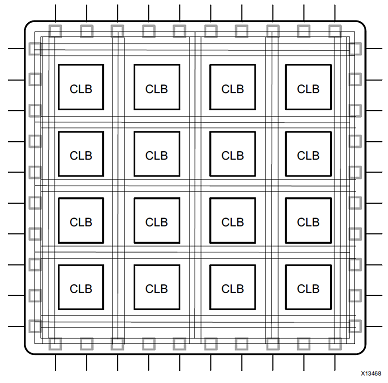
\includegraphics[scale=0.7]{fpga.png}
\caption{Xilinx FPGA \cite{xilinx:2017}}
\label{fig:FPGA}
\end{figure}
\section{Hardware Description Languages}


The CLBs in this architecture are comprised of LUTs and Flip-Flops, in order to implement boolean functions and allow the design of synchronous circuits. FPGAs produced by Xilinx are mostly SRAM based, other approaches are flash or anti-fuse based architectures.